\documentclass{beamer}

%% For code listings
\usepackage{minted} 

\usetheme{metropolis}

\begin{document}
\title{Reinforcement Learning}
\subtitle{A Hands On Introduction}
\frame{\titlepage}

\section{Introduction}
\begin{frame}
  \frametitle{todo}
  \tableofcontents[currentsection]
\end{frame}

\begin{frame}
  \frametitle{The Case for RL}
  \begin{center}
    \hspace{-1.0cm}
    \vspace{-2.0cm}
    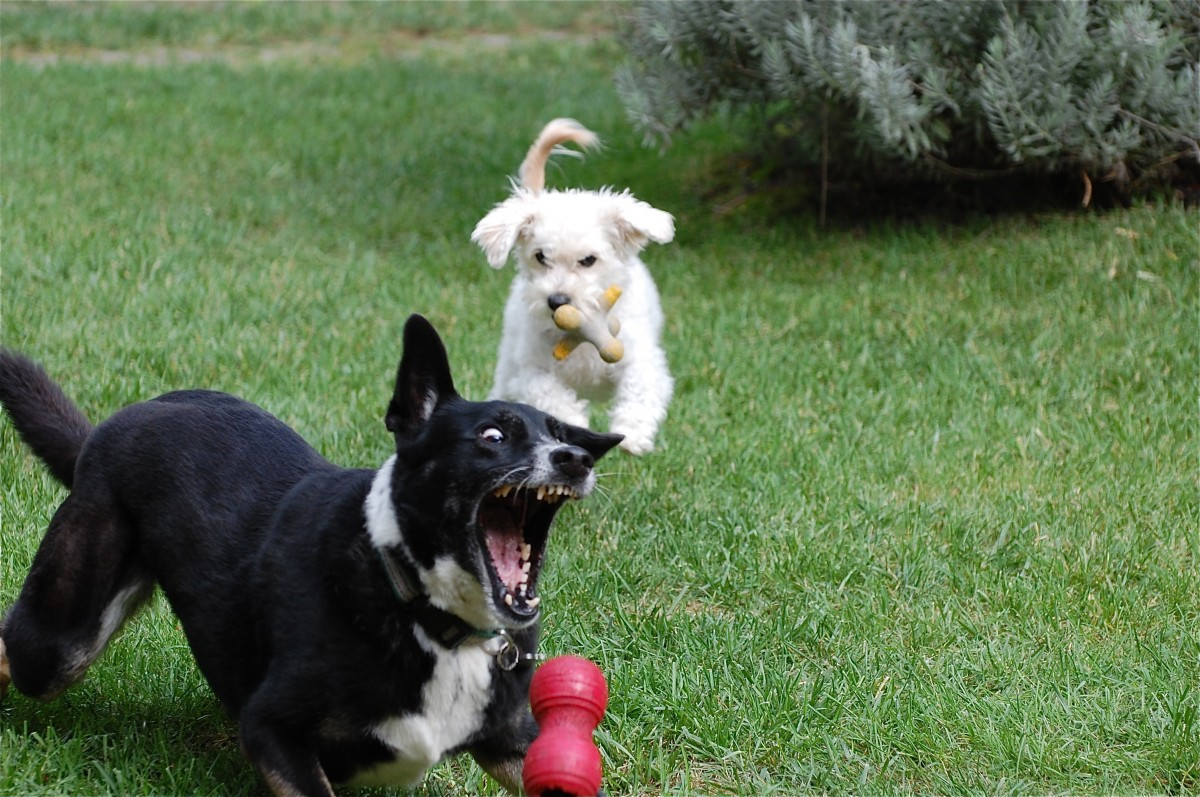
\includegraphics[scale=0.4]{assets/dog.jpg}
  \end{center}

\end{frame} 

\begin{frame}
  \frametitle{RL in a Nutshell}
  \begin{itemize}
  \item Dynamic
  \item Uncertain
  \item Exploration
  \item Delayed consequences
  \item Rquires planning
  \end{itemize} 
\end{frame}



\section{Funciton Approximator}


\begin{frame}
  \frametitle{This is the second slide}
  \framesubtitle{A bit more information about this}
\end{frame}

\section{Bellman Equaiton}
\begin{frame}
  \frametitle{Updating our world view}
  \framesubtitle{A bit more information about this}
  \begin{block}{hello}
    \inputminted[firstline=21, lastline=22, autogobble,breaklines]{python}{../updates.py}
  \end{block}
\end{frame}
\end{document}